
%% bare_jrnl_compsoc.tex
%% V1.4a
%% 2014/09/17
%% by Michael Shell
%% See:
%% http://www.michaelshell.org/
%% for current contact information.
%%
%% This is a skeleton file demonstrating the use of IEEEtran.cls
%% (requires IEEEtran.cls version 1.8a or later) with an IEEE
%% Computer Society journal paper.
%%
%% Support sites:
%% http://www.michaelshell.org/tex/ieeetran/
%% http://www.ctan.org/tex-archive/macros/latex/contrib/IEEEtran/
%% and
%% http://www.ieee.org/

%%*************************************************************************
%% Legal Notice:
%% This code is offered as-is without any warranty either expressed or
%% implied; without even the implied warranty of MERCHANTABILITY or
%% FITNESS FOR A PARTICULAR PURPOSE! 
%% User assumes all risk.
%% In no event shall IEEE or any contributor to this code be liable for
%% any damages or losses, including, but not limited to, incidental,
%% consequential, or any other damages, resulting from the use or misuse
%% of any information contained here.
%%
%% All comments are the opinions of their respective authors and are not
%% necessarily endorsed by the IEEE.
%%
%% This work is distributed under the LaTeX Project Public License (LPPL)
%% ( http://www.latex-project.org/ ) version 1.3, and may be freely used,
%% distributed and modified. A copy of the LPPL, version 1.3, is included
%% in the base LaTeX documentation of all distributions of LaTeX released
%% 2003/12/01 or later.
%% Retain all contribution notices and credits.
%% ** Modified files should be clearly indicated as such, including  **
%% ** renaming them and changing author support contact information. **
%%
%% File list of work: IEEEtran.cls, IEEEtran_HOWTO.pdf, bare_adv.tex,
%%                    bare_conf.tex, bare_jrnl.tex, bare_conf_compsoc.tex,
%%                    bare_jrnl_compsoc.tex, bare_jrnl_transmag.tex
%%*************************************************************************


% *** Authors should verify (and, if needed, correct) their LaTeX system  ***
% *** with the testflow diagnostic prior to trusting their LaTeX platform ***
% *** with production work. IEEE's font choices and paper sizes can       ***
% *** trigger bugs that do not appear when using other class files.       ***                          ***
% The testflow support page is at:
% http://www.michaelshell.org/tex/testflow/


\documentclass[10pt,conference,onecolumn,compsoc]{IEEEtran}


\usepackage{hyperref}
\usepackage{enumitem}
\setlist[itemize]{leftmargin=3 cm}
\setlist[enumerate]{leftmargin=3cm}



% *** CITATION PACKAGES ***
%
\ifCLASSOPTIONcompsoc
  % IEEE Computer Society needs nocompress option
  % requires cite.sty v4.0 or later (November 2003)
  \usepackage[nocompress]{cite}
\else
  % normal IEEE
  \usepackage{cite}
\fi
% cite.sty was written by Donald Arseneau
% V1.6 and later of IEEEtran pre-defines the format of the cite.sty package
% \cite{} output to follow that of IEEE. Loading the cite package will
% result in citation numbers being automatically sorted and properly
% "compressed/ranged". e.g., [1], [9], [2], [7], [5], [6] without using
% cite.sty will become [1], [2], [5]--[7], [9] using cite.sty. cite.sty's
% \cite will automatically add leading space, if needed. Use cite.sty's
% noadjust option (cite.sty V3.8 and later) if you want to turn this off
% such as if a citation ever needs to be enclosed in parenthesis.
% cite.sty is already installed on most LaTeX systems. Be sure and use
% version 5.0 (2009-03-20) and later if using hyperref.sty.
% The latest version can be obtained at:
% http://www.ctan.org/tex-archive/macros/latex/contrib/cite/
% The documentation is contained in the cite.sty file itself.



% *** GRAPHICS RELATED PACKAGES ***
%
\ifCLASSINFOpdf
   \usepackage[pdftex]{graphicx}
 
\else
 
\fi
% graphicx was written by David Carlisle and Sebastian Rahtz. It is
% required if you want graphics, photos, etc. graphicx.sty is already
% installed on most LaTeX systems. The latest version and documentation
% can be obtained at: 
% http://www.ctan.org/tex-archive/macros/latex/required/graphics/
% Another good source of documentation is "Using Imported Graphics in
% LaTeX2e" by Keith Reckdahl which can be found at:
% http://www.ctan.org/tex-archive/info/epslatex/
%
% latex, and pdflatex in dvi mode, support graphics in encapsulated
% postscript (.eps) format. pdflatex in pdf mode supports graphics
% in .pdf, .jpeg, .png and .mps (metapost) formats. Users should ensure
% that all non-photo figures use a vector format (.eps, .pdf, .mps) and
% not a bitmapped formats (.jpeg, .png). IEEE frowns on bitmapped formats
% which can result in "jaggedy"/blurry rendering of lines and letters as
% well as large increases in file sizes.
%
% You can find documentation about the pdfTeX application at:
% http://www.tug.org/applications/pdftex









% *** PDF, URL AND HYPERLINK PACKAGES ***
%
\usepackage{url}
% url.sty was written by Donald Arseneau. It provides better support for
% handling and breaking URLs. url.sty is already installed on most LaTeX
% systems. The latest version and documentation can be obtained at:
% http://www.ctan.org/tex-archive/macros/latex/contrib/url/
% Basically, \url{my_url_here}.




\begin{document}

\title{Music Manager}
%
%

% received ..."  text while in non-compsoc journals this is reversed. Sigh.

\author{Andrew Marshall, Kyle Rolland\\% <-this % stops a space
}

\IEEEtitleabstractindextext{%
\begin{abstract}
The goal of this project is to create an interface that allows a user to store and manage music on their machine. Users will be able to create play lists, favorite certain songs, and sort songs by the artist, or the song name. Our goal with this project is to make a simple version of music applications like Spotify or iTunes, for people who don't like using their current music player application.
\end{abstract}

}


% make the title area
\maketitle



\IEEEdisplaynontitleabstractindextext

\IEEEpeerreviewmaketitle



\section{Introduction}


Music is an everyday part of life, and many people go everyday without even thinking about the luxury that we have in the modern era, being able to listen to what we want, wherever we want to. Following this, there are many many platforms that one can use to access music. We aim to reproduce one such platform, creating an interface that allows someone to add music of their choosing, organize it, and play it. 
	
Providing people with more options is never a bad thing. Even if there are only a few things that differentiate one software from another, there are always going to be users looking for new experiences. We would like to be able to appeal to as wide an audience as possible, people who have problems with the existing flaws in other software, which are ignored or put off of being fixed by developers. Helping those people find a new place where they feel they can store their favorite songs can make a large difference, especially because music can be a very valuable, memorable resource for some people.

\subsection{Background}
Over the course of this proposal, we will use the term Metadata, and in this case, it's really just a technical term for basic music information. It pertains to things like album art, release date, track/song length, genre, artist, and the songs title.

We decided on a project like this because music is something that is easy to make connections between. Thankfully, The two of us had common ground in a genre that we used to listen to, but even if we didn't, it would be easy to come together to work on a project like this. It originally sprouted as an idea for an audio waveform visualizer, the flashing bars/lights that you'll see with music videos, that correspond to the beat of the song, or the lyrics. Neither of us have looked into what it takes to make those, and some further consideration led us to decide that it would be better to take a step back and just make a music management interface.

Andrew has run into problems with CDs on iTunes, so we hope to be able to implement a way transfer music from the manager to the CD, allowing the manager to effectively use and read CDs.

Kyle's main music application is Apple Music , and he has some issues with listening queue management, for example, shuffling a play list, and then adding it to the end of the list of what is currently being listened to, which is not possible in the application. If we could work the capability into this project, it may become an alternative listening application for him as well.

\subsection{Impacts}
There are many music managing systems on the internet, and we would like to see if we can create something worth telling others about, so that they can use as well. We want to add some functionality that gives us a chance to stand out, making it easier to reach even just a few people, and give them another place to handle the songs that they hold dear. It doesn't take much to brighten someone's day, and hopefully with this project we can manage to do that for a handful of people.

\subsection{Challenges}
It may be difficult to organize and handle the previously mentioned metadata, since there is a lot of information that goes along with it. We also may run into trouble trying to create a system to accept different file types, like .mp3 versus .mp4 versus .wav, but working a system like this out would prove very useful for attracting more users. Making a display for things like album art, and giving the user the option to upload their own art to go with songs or created play lists may also prove to be difficult, partially because of accepting images, and partially reaching back to accepting different image file types, like .jpeg and .png. Lastly, we are still sort of hoping to implement an audio waveform visualizer somewhere within the interface, and we think this will prove to be the biggest hurdle, especially if we can't find a framework to start with.


\section{Scope}
Our project will be completed when we have an interface that allows the user to add songs of their choosing, modify their metadata, add those songs to play lists and edit those play lists freely and easily, search for songs within their database, and sort them by given data types, like artist, genre, and song title

We have some ideas for stretch goals. One of them would be implementing the previously mentioned audio waveform visualizer. Along with this, being able to easily export your play lists or songs to various different platforms would be very handy. Lastly, we would love to be able to implement a system that allows the user to upload images for artwork that will display when a song is playing, be it album art, or an image that will act as the cover of a given play list, allowing for more user customization.

\subsection{Requirements}
To decide on the requirements for our project, the two of us sat down and discussed the basics of what we needed to consider the application to be acceptable. Making a play list, adding and removing songs, and implementing a listening queue are a few examples. They are signified by having a priority of 1 in the use case table (See Table \ref{tab:useCaseIndex}). Afterwards, we talked about what we thought we be useful or unique features to try and include, which are signified by 2's and 3's in the table, depending on how important including them was.

\subsubsection{Functional}
\begin{itemize}
\item Store songs that are currently being played, and are queued to play
\item Keep track of previously played songs for accessibility later
\item Display current song being played, as well as associated artwork
\item Hold songs that are being played for storage across listening sessions
\item Give access to specific metadata, like genre or song name, allowing user to make changes
\item Allow for customization of user created play lists
\item Prevent duplication of music in library
\item Import/export songs from CD
\item Adhere to copyright laws, recognizing proper credit to musicians 
\end{itemize}

\subsubsection{Non-Functional}
\begin{itemize}
\item When user updates music information, efficiently adjust related processes
\item Ensure that music and image files are of proper file formatting
\item Ensure that songs and data are easily accessible and understandable to the user, through effective use of application interface
\end{itemize}

\subsection{Use Cases}
Use Case index can be seen in Table \ref{tab:useCaseIndex}.




\begin{table}
\centering
\begin{tabular}{|c|c|c|c|c|}
\hline
Use Case ID & Use Case Name & Primary Actor & Complexity & Priority \\
\hline \hline
1 & Add song to queue & Listener & Med & 1\\
\hline
2 & Add new song to manager & Listener & Hard & 1\\
\hline
3 & Add album art & Listener & Med & 2\\
\hline
4 & Play from CD & Listener & Hard & 3\\
\hline
5 & Change volume & Listener & Med & 1\\
\hline
6 & Modify data & Listener & Easy & 2\\
\hline
7 & Remove song & Listener & Med & 2\\
\hline
8 & Play play list & Listener & Easy & 1\\
\hline
9 & Save play list & Listener & Med & 1\\
\hline
10 & Edit play list & Listener & Med & 1\\
\hline
11 & Display album art & Listener & Med & 1\\
\hline

\end{tabular}
\caption{Use case index}
\label{tab:useCaseIndex}
\end{table}


\begin{itemize}
\item[Use Case Number:] 1
\item[Use Case Name:] Add song to queue
\item[Description:] User selects a song that they wish to play next. They will click on a plus button that appears when hovering over the song. This will add the song to the bottom of the list.
\end{itemize}

\begin{enumerate}
\item User selects song that they want to play next
\item After selecting song, plus button appears on song bar
\item User presses button, adds song to queue
\item[Termination Outcome:] Selected song will be played next
\end{enumerate}

(see Figure \ref{AddSong})

\begin{itemize}
\item[Use Case Number:] 2
\item[Use Case Name:] Add music to manager
\item[Description:] Menu bar at top of screen will have a file button. User presses button, and asks user what they would like to add. User selects song, asks for file name of song that will be added. If file can be found, and is an accepted file type, it will be added to the manager.
\end{itemize}

\begin{enumerate}
\item User presses File button on menu bar
\item Drop down menu appears, allows user to click on Add Song...
\item User enters song file that they want to add
\item If file is appropriate formatting, song is added to manager
\item [Termination Outcome:] New song is present in management library
\end{enumerate}

Alternatively:
\begin{enumerate}
\item User presses File button on menu bar
\item Drop down menu appears, allows user to click Add Song...
\item User enters song file that they want to add
\item Song is already in library
\item Song is prevented from being added
\item (OPTIONAL: Sends user to song in library once prevention occurs)
\item [Termination Outcome:] Duplication of song(s) prevented
\end{enumerate}

(see Figure \ref{AddMusic})

\begin{itemize}
\item[Use Case Number:] 3
\item[Use Case Name:] Add album art
\item[Description:] When looking at an album or play list, displays a button that will allow the user to select an image to upload. Once selected, image will be used as art for the given album/play list.
\end{itemize}

\begin{enumerate}
\item User opens album or play list
\item User presses button at top corner of album art area
\item Menu appears that allows user to modify item
\item User selects Add Image...
\item User enters image name that they would like
\item If file is appropriate formatting, art is replaced
\item [Termination Outcome:] Previous album art is replaced with new art
\end{enumerate}

(see Figure \ref{AddAlbumArt})

\begin{itemize}
\item[Use Case Number:] 4
\item[Use Case Name:] Play from CD
\item[Description:] Menu bar at top of screen will have a device button, clicking on it allows user to select a CD to play music from, or send music to.
\end{itemize}

\begin{enumerate}
\item User presses Device button on menu bar
\item Drop down menu appears
\item User selects Import from CD
\item Music on CD is loaded into manager
\item [Termination Outcome:] Music present on CD is now loaded into user's library
\end{enumerate}

(See Figure \ref{PlayCD})

\begin{itemize}
\item[Use Case Number:] 5
\item[Use Case Name:] Change volume
\item[Description:] Volume buttons displayed beneath play section (Possibly replace with volume slider/better display). User presses + button to increment volume up by one, and - button to decrement volume by one, to an upper and lower limit respectfully.
\end{itemize}

\begin{enumerate}
\item User presses plus button next to speaker image
\item [Termination Outcome:] Volume increases by one increment
\end{enumerate}

Alternatively:
\begin{enumerate}
\item User presses minus button next to speaker image
\item [Termination Outcome:] Volume decreases by one increment
\end{enumerate}

(See Figure \ref{VolumeButton})

\begin{itemize}
\item[Use Case Number:] 6
\item[Use Case Name:] Modify Data
\item[Description:] Allows user to change metadata tied to the selected song, giving the ability to change things like song genre or song name
\end{itemize}

\begin{enumerate}
\item User right clicks song that they would like to modify
\item Information about song is displayed in boxes
\item User can manually enter information that would not affect copyright
\item User can then save changes to song
\item[Termination Outcome:] Song information is changed to what the user would like
\end{enumerate}

\begin{itemize}
\item[Use Case Number:] 7
\item[Use Case Name:] Remove Song
\item[Description:] Allows user to remove a song from the manager, and updates the manager accordingly
\end{itemize}

\begin{enumerate}
\item User selects song that they would like to delete
\item User clicks the delete button
\item Song is removed from song list
\item Display is updated so that the song no longer appears
\item[Termination Outcome:] Song is removed from list and song display
\end{enumerate}

\begin{itemize}
\item[Use Case Number:] 8
\item[Use Case Name:] Play play list
\item[Description:] User selects the play list that that they would like to play. The songs are then loaded and played
\end{itemize}

\begin{enumerate}
\item User clicks load play list
\item User selects play all
\item Manager will play all songs in play list, transitioning between songs automatically
\item[Termination Outcome:]	Play list is loaded, and user can play the songs in it
\end{enumerate}

\begin{itemize}
\item[Use Case Number:] 9
\item[Use Case Name:] Save play list
\item[Description:] Allows user to save songs in list as a play list, which can be loaded and played later
\end{itemize}

\begin{enumerate}
\item User loads songs into song list, in order they want in the play list
\item User clicks Save Playlist
\item[Termination Outcome:] Songs loaded are saved as a play list for later listening
\end{enumerate}

\begin{itemize}
\item[Use Case Number:] 10
\item[Use Case Name:] Edit play list
\item[Description:] User can change the order of songs, add songs, or remove songs to the selected play list
\end{itemize}

\begin{enumerate}
\item User selects play list to load
\item Play list is loaded
\item User presses edit play list button
\item User can then change song order, remove songs, or add songs
\item[Termination Outcome:] Play list is updated with the user's changes
\end{enumerate}

\begin{itemize}
\item[Use Case Number:] 11
\item[Use Case Name:] Display Album Art
\item[Description:] Songs that have corresponding art will display the art when played
\end{itemize}

\begin{enumerate}
\item User selects song to be played
\item User presses play button
\item Art tied to song is displayed while song is selected
\item[Termination Outcome:] Art for chosen song is displayed on screen 
\end{enumerate}

\subsection{Interface Mockups}
Included below are some basic ideas for what the user will see in the program. Starting off, we have 2 ideas for how the interface could look, inspired by some already existing music player applications (See Figure \ref{Interface1}, Figure \ref{Interface2}). Following those are plans for how certain user interaction will look. First is adding a song to the song queue (See Figure \ref{AddSong}), which would be accessed by hovering over a song. Next, we have a mock up of how the user would add a song to the manager (See Figure \ref{AddMusic}), by pressing a file button, giving the user the choice to add songs. The next figure is an idea of what it may look like when the user wants to tie an image to a song (See Figure \ref{AddAlbumArt}), a small button will appear that will open the file explorer when clicked, where the user can select an image to link to a song. After, we have a mock up of what the menu for interacting with a CD or other outside device may look like (See Figure \ref{PlayCD}), which would function in a similar manner to the file drop down box, but with options specific to outside devices.. The last figure shows an option for volume control (See Figure \ref{VolumeButton}), where there will be simple plus and minus buttons that would adjust the volume by specific increments until a minimum or maximum is reached.

\begin{figure}[ht!]
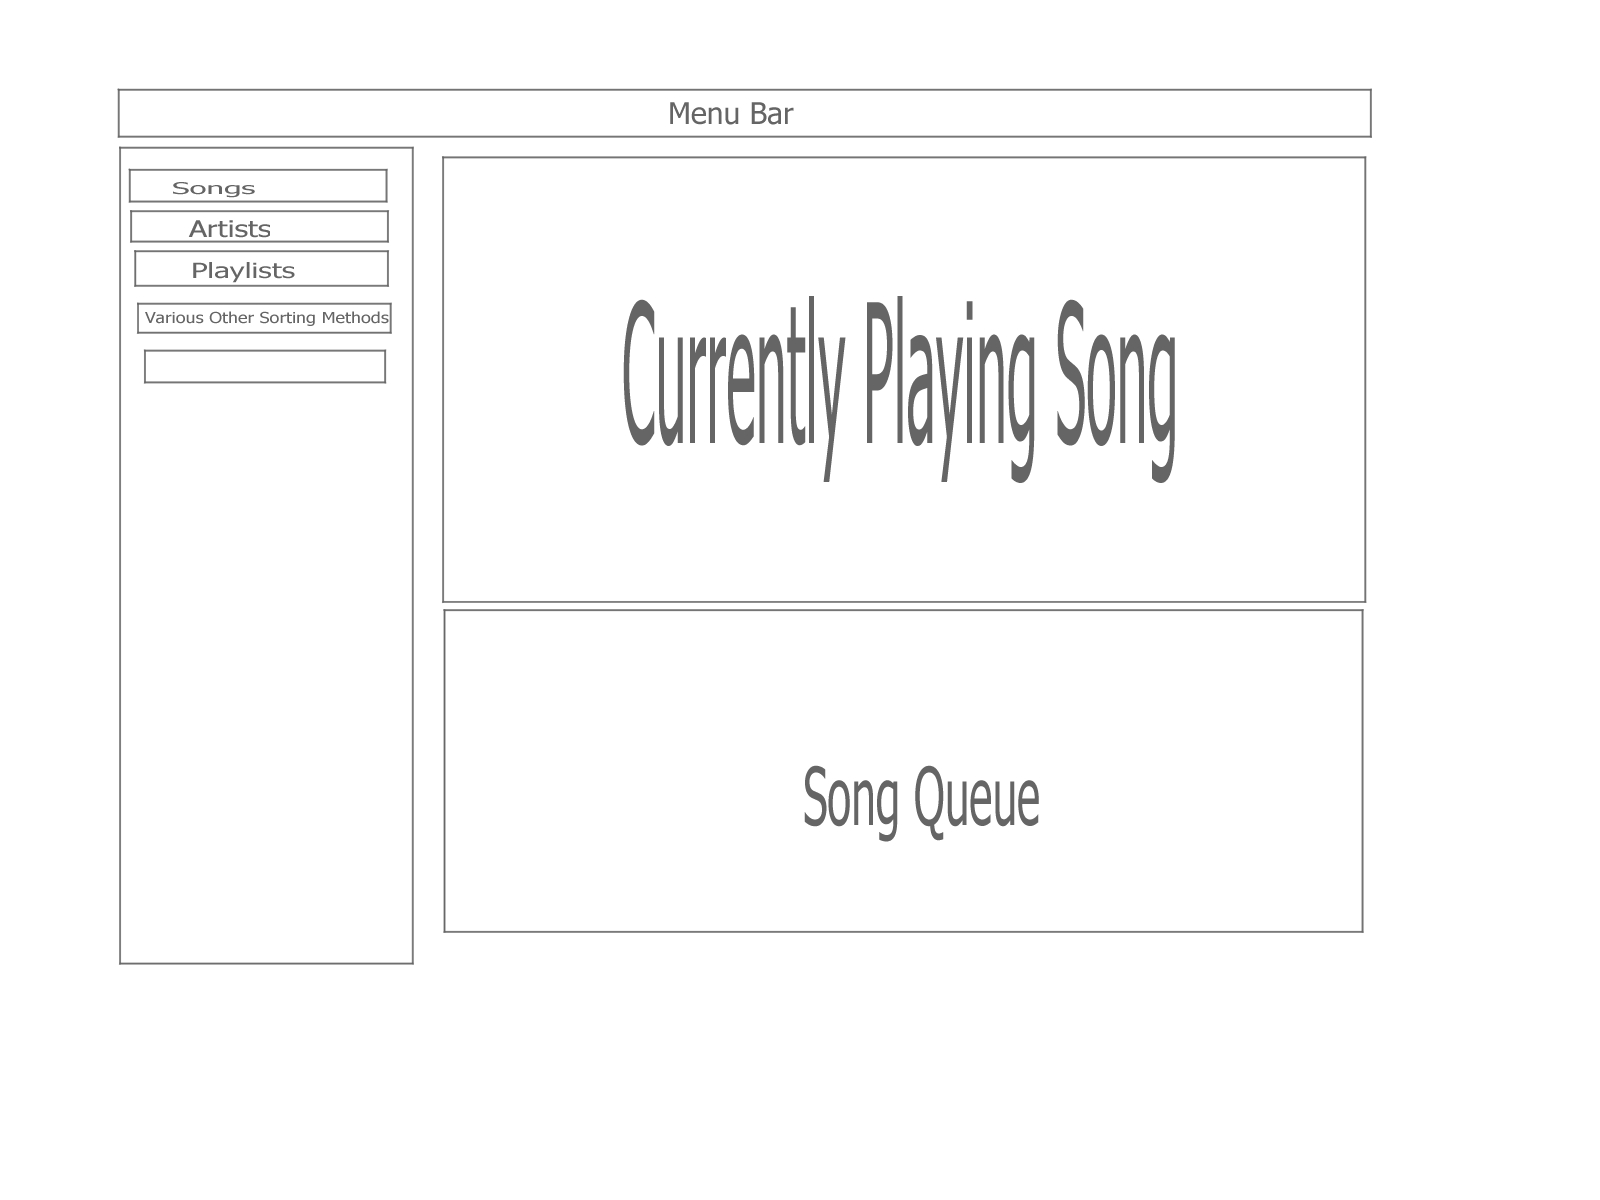
\includegraphics[height=200px, width=250px]{Interface_Mock_Up_1.jpg}
\caption{Interface Idea 1, Sorting options are located on left, current song in center, song queue always displayed beneath current song}
\label{Interface1}
\end{figure}

\begin{figure}
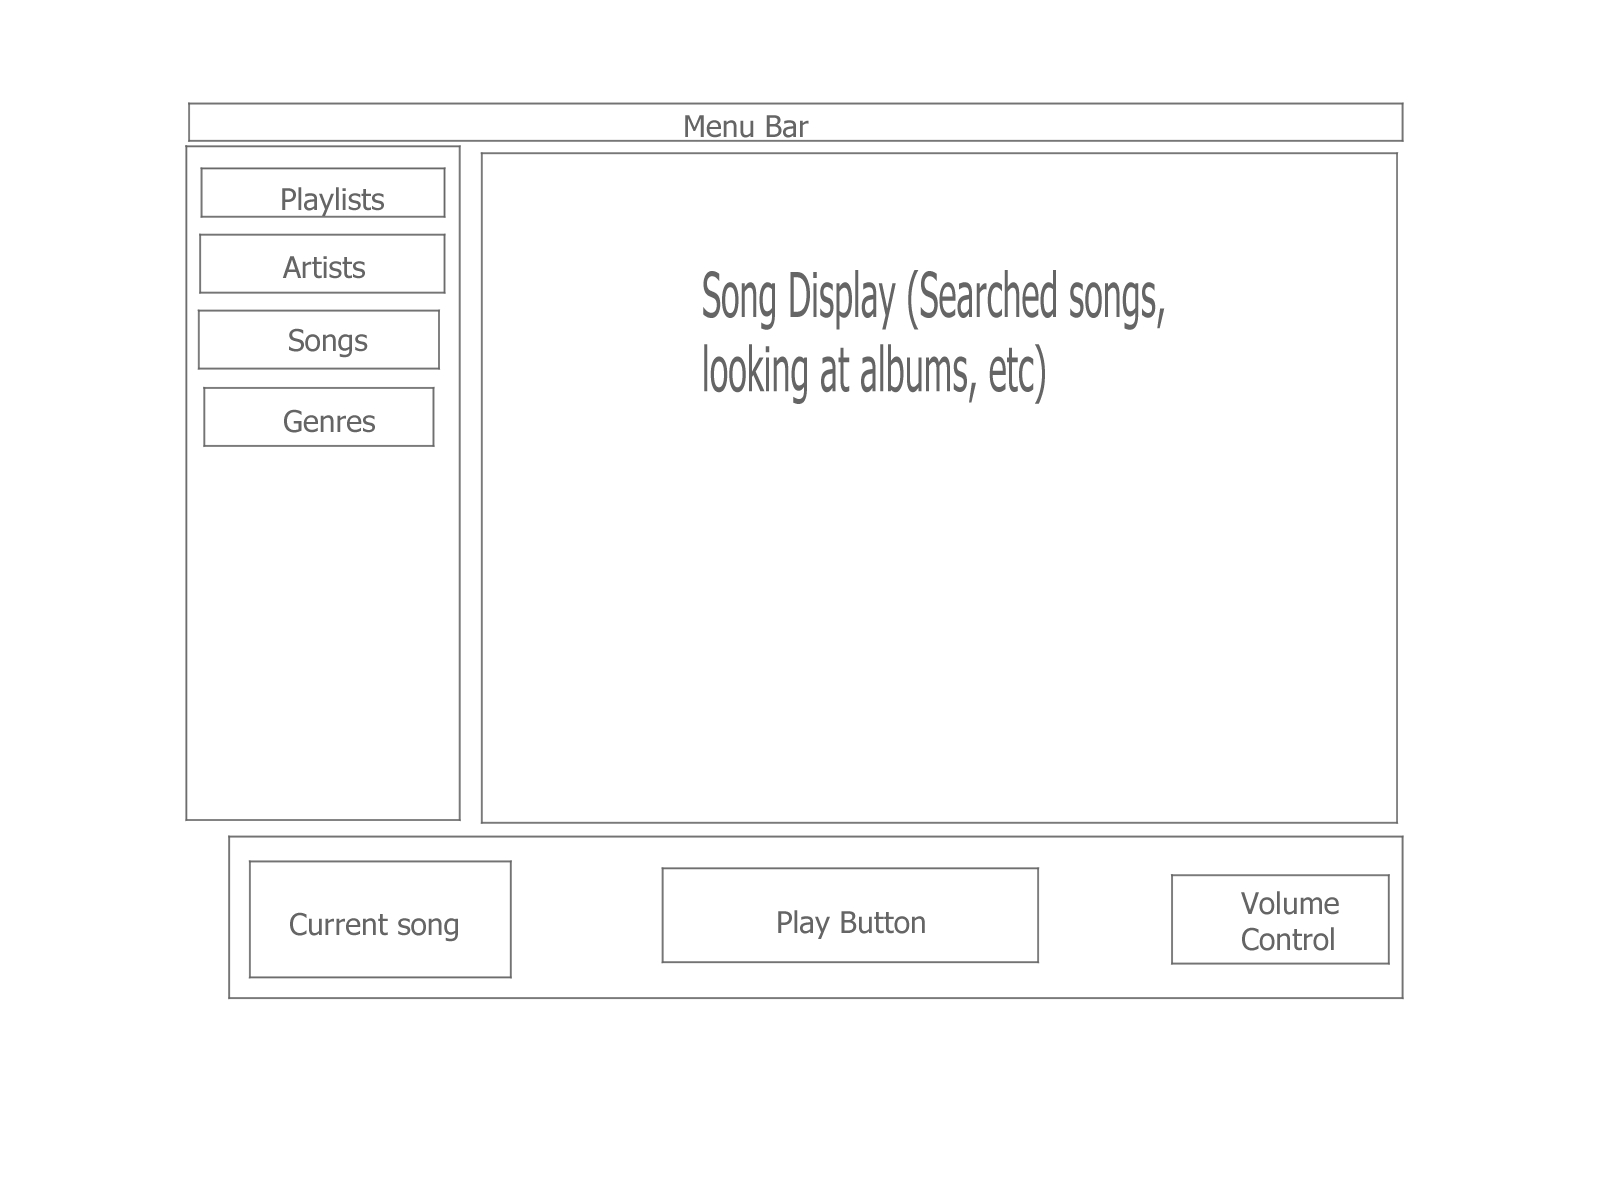
\includegraphics[height=200px, width=250px]{Interface_Mock_Up_2.jpg}
\caption{Interface Idea 2, Sorting options located on left, large display for library/searches, smaller concise play area with buttons for volume and song queue}
\label{Interface2}
\end{figure}

\begin{figure}[ht!]
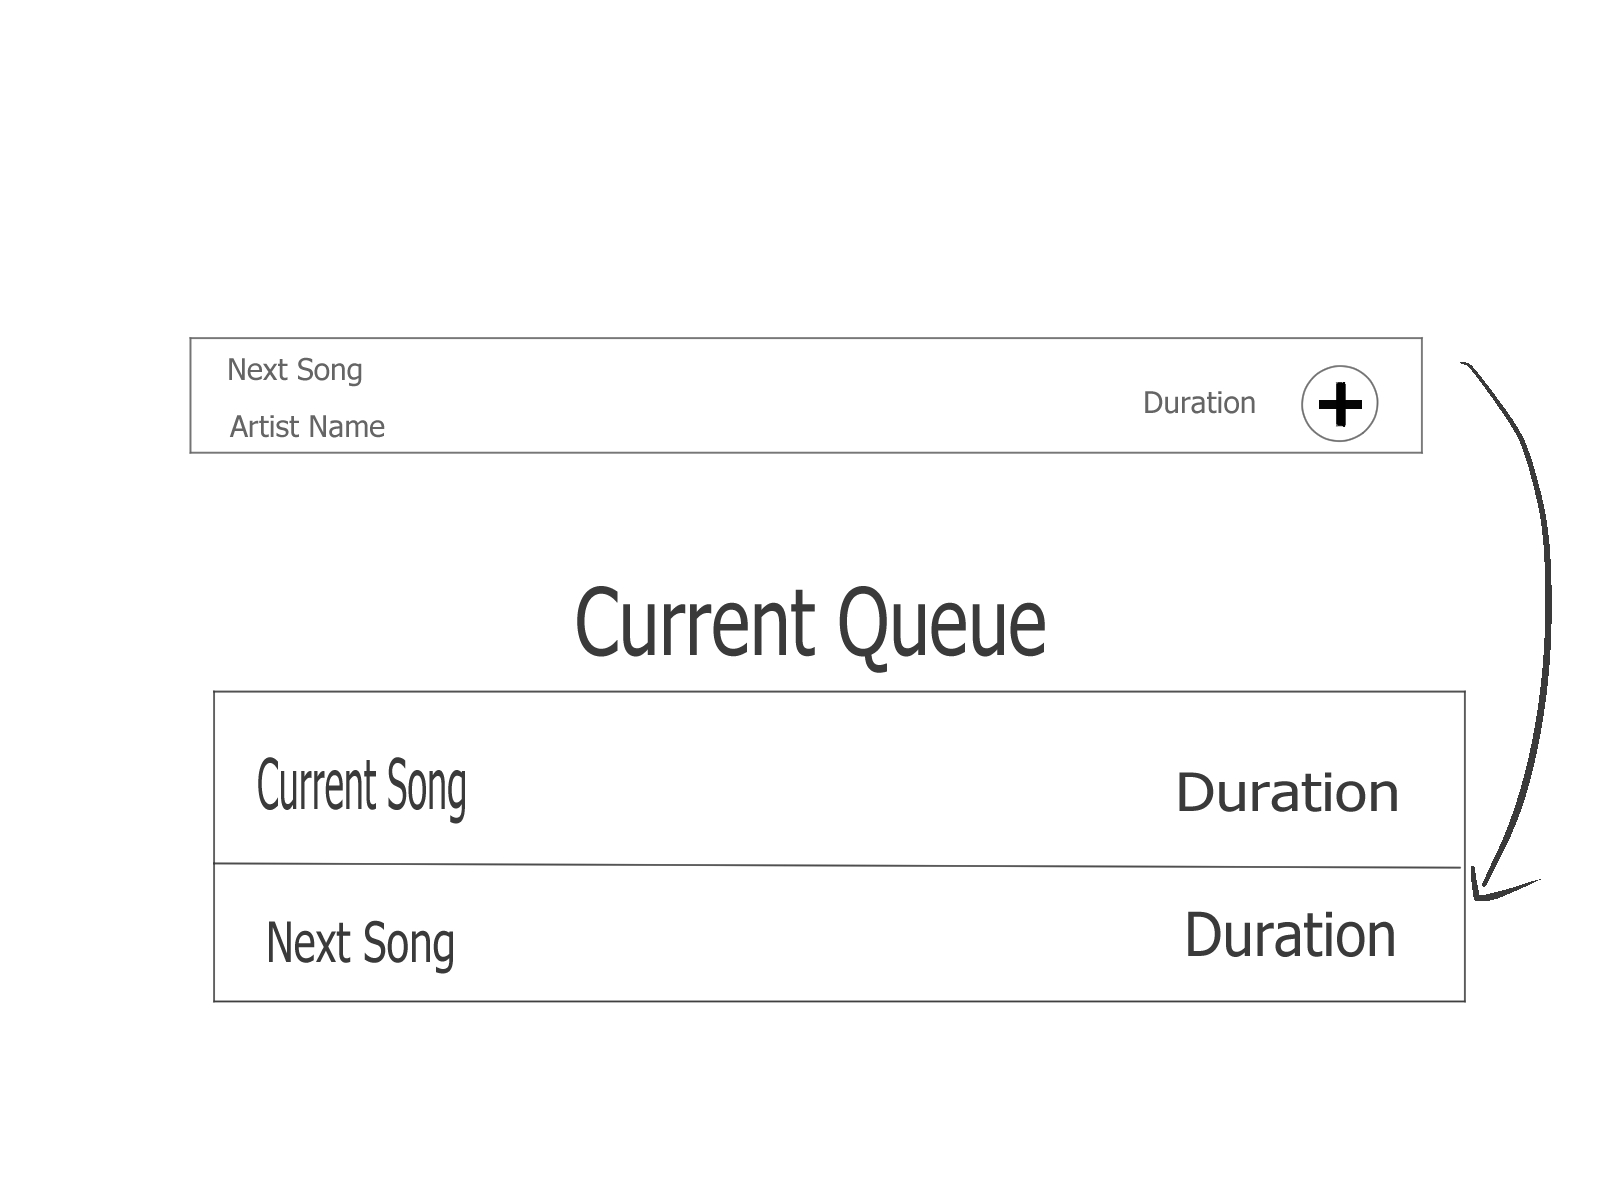
\includegraphics[height=200px, width=250px]{Add_Song_Queue_Mock_Up.jpg}
\caption{Use Case 1, Adding song to queue, When hovering over a song, a plus button appears, pressing the button will add the song to the top of the song list, to be played next}
\label{AddSong}
\end{figure}

\begin{figure}[ht!]
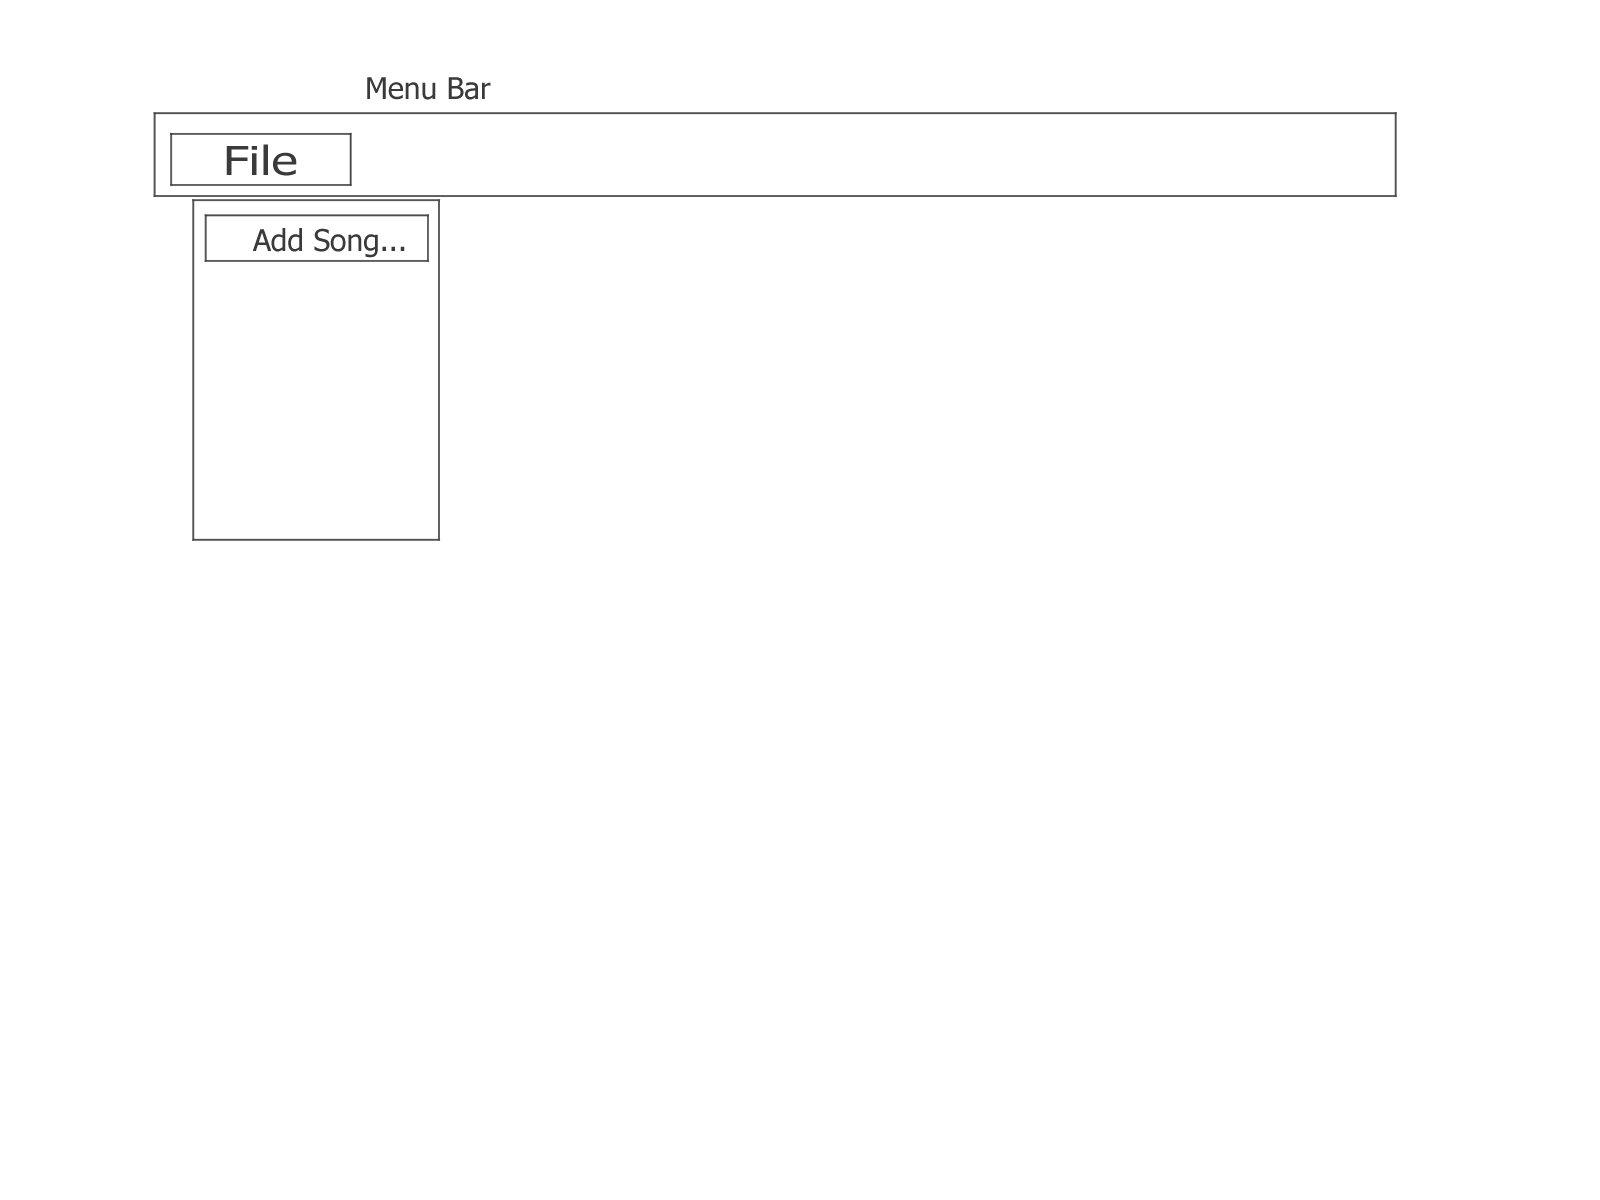
\includegraphics[height=150px, width=250px]{Add_Music_Mock_Up.jpg}
\caption{Use Case 2, Adding music to manager, File button located first on the menu bar, pressing it opens the file options, clicking "Add Song" at top opens window and allows user to select the song they wish to add}
\label{AddMusic}
\end{figure}

\begin{figure}
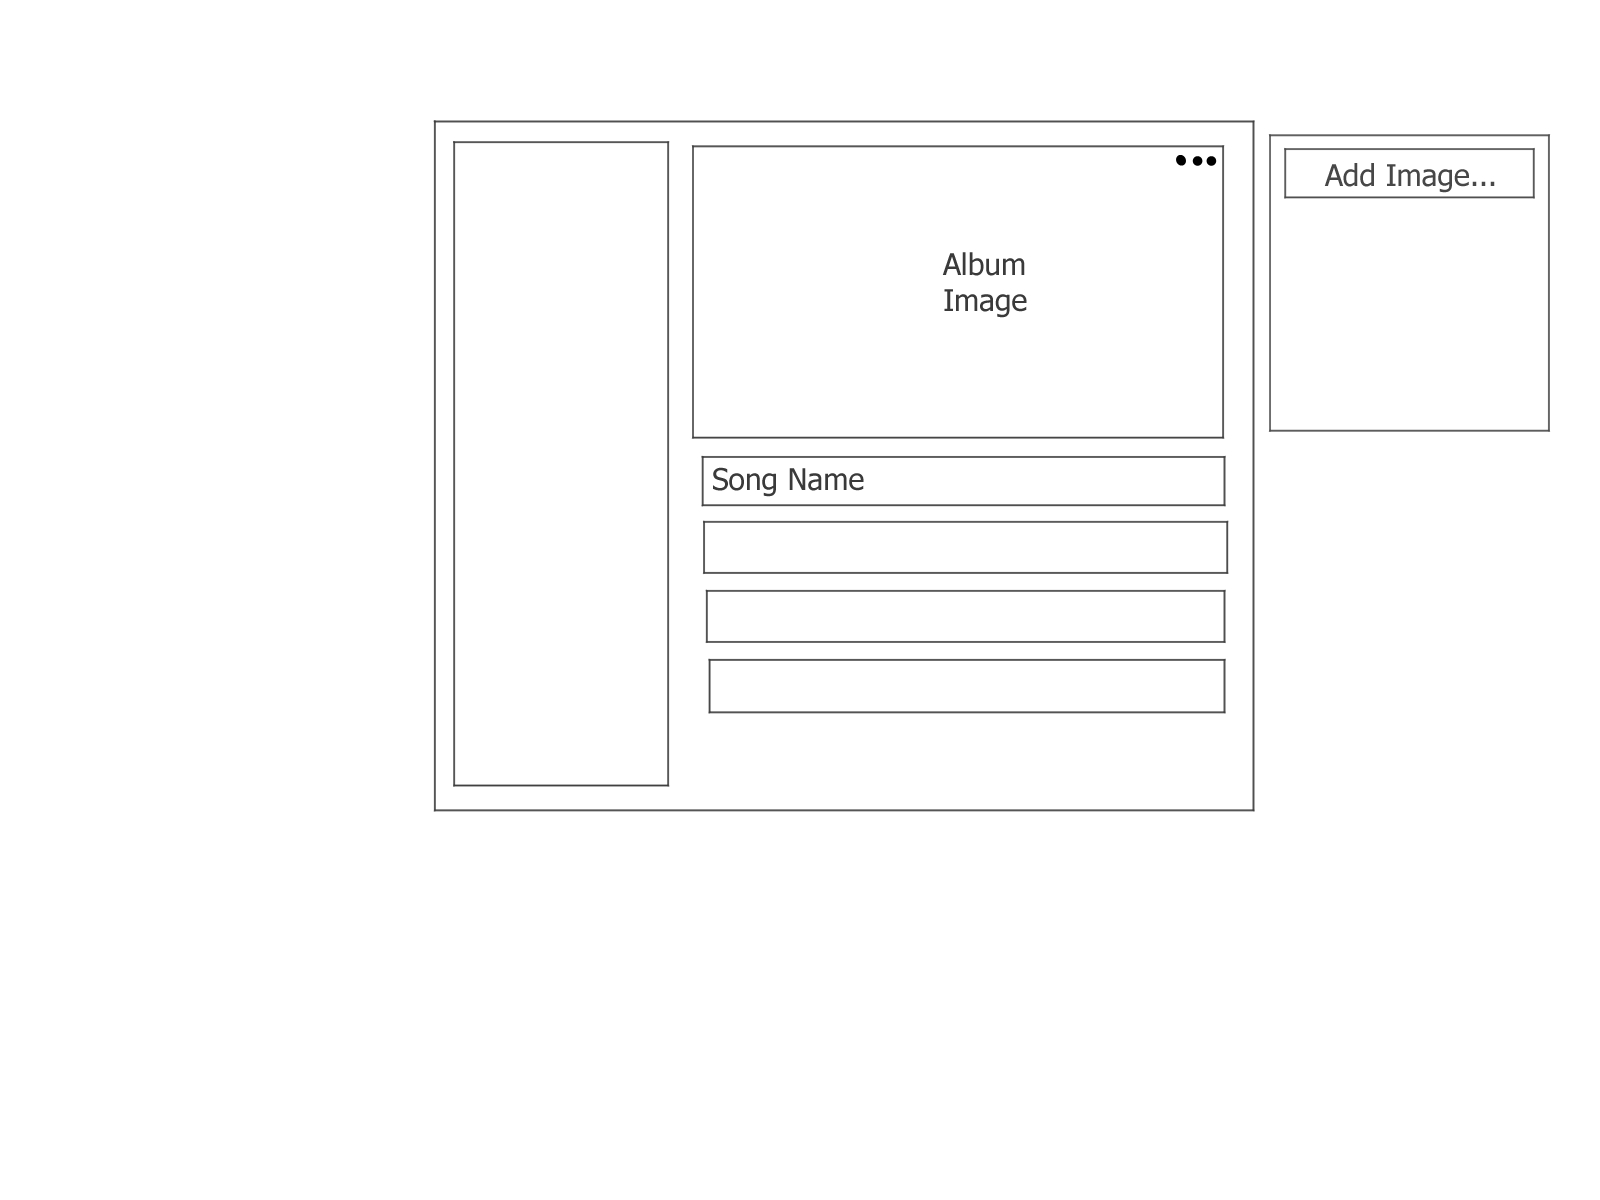
\includegraphics[height=200px, width=250px]{Add_Image_Mock_Up.jpg}
\caption{Use Case 3, Adding album art, 3 dots at top open menu when clicked, clicking add image allows user to select an image that will be use for the album}
\label{AddAlbumArt}
\end{figure}

\begin{figure}
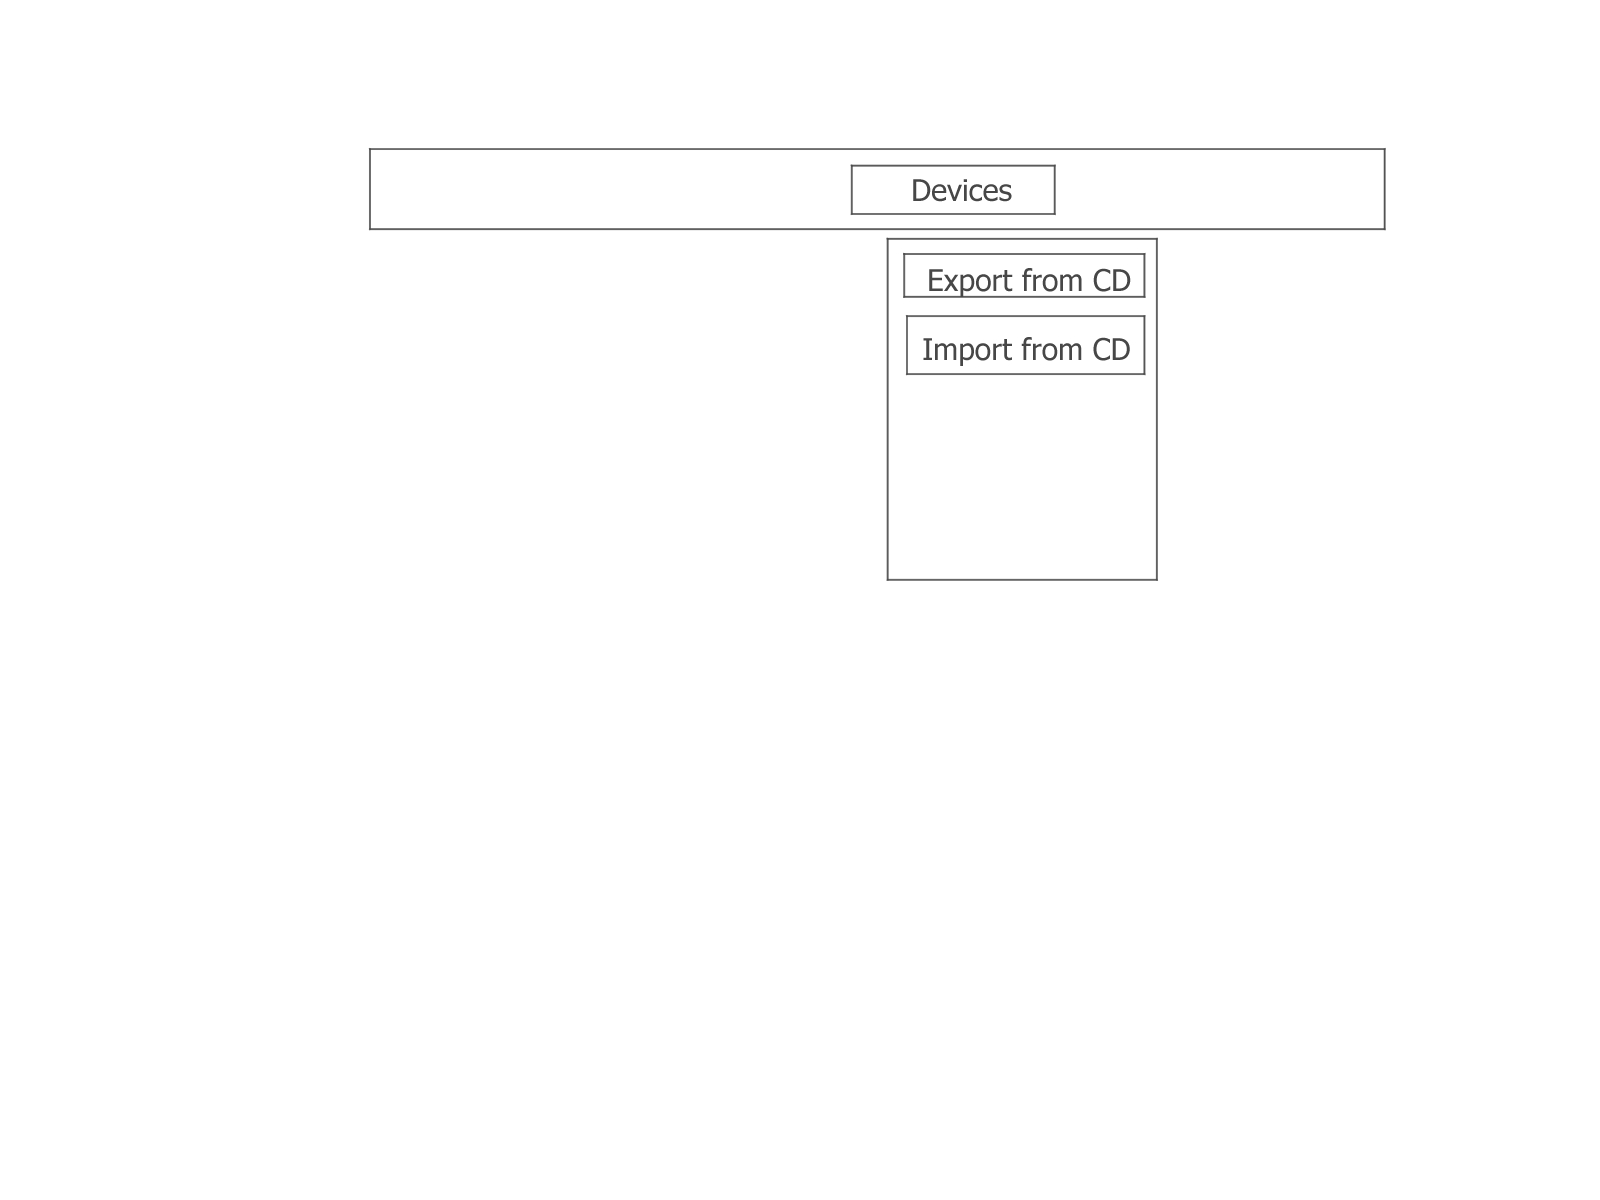
\includegraphics[height=150px, width=250px]{Play_CD_Mock_Up.jpg}
\caption{Use Case 4, Interacting with CD, Device button on menu car, clicking it opens drop down menu with 2 buttons, one for importing songs into the library from a CD, and the other for exporting songs to the CD from the library}
\label{PlayCD}
\end{figure}

\begin{figure}
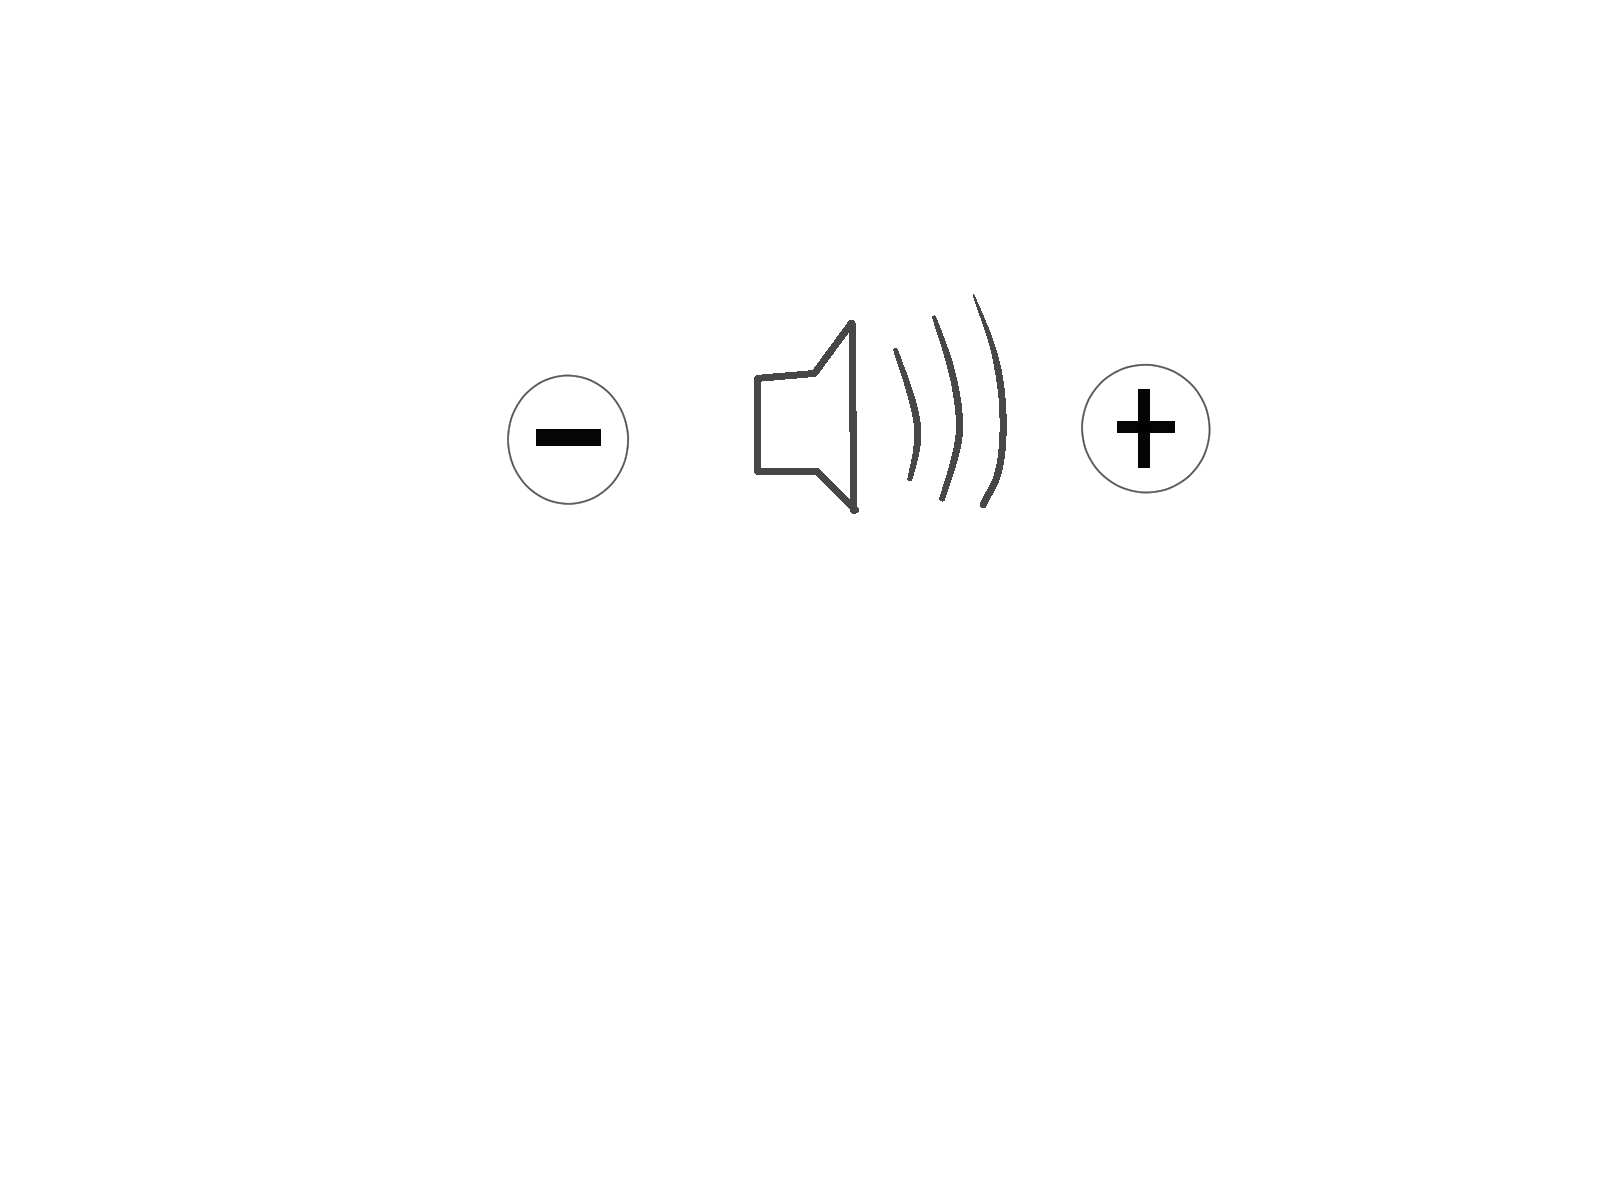
\includegraphics[height=150px, width=250px]{Volume_Button_Mock_Up.jpg}
\caption{Use Case 5, Volume button, Plus and minus buttons on each side of the volume icon, pressing plus increments volume by one, pressing down decrements volume by one}
\label{VolumeButton}
\end{figure}

\section{Project Timeline}
\begin{enumerate}
\item Project topic decided - January 30, 2021
\item Project proposal draft due - February 1, 2021
\item First project proposal update due - February 12, 2021
\item UML of project created - March 10, 2021
\item Second project proposal update due - March 19, 2021
\item Create usable song class - March 25, 2021
\item test song class - March 30, 2021
\item Create working album class - April 4, 2021
\item Create working play list class - April 9, 2021
\item Create and test file, volume, pause/play buttons - April 14, 2021
\item Create working queue class - April 19, 2021
\item Create and test navigation and skip buttons - April 24, 2021
\item Project ready to be demonstrated - April 29, 2021
\end{enumerate}

\section{Project Structure}
The manager will be designed to keep things as simple as possible, which is both useful for the users, and easier on us for programming. As we started working on the application, we realized that we could simplify some things for an easier experience while programming, while not sacrificing anything that the user would experience, which we decided to try and take advantage of.

For example, we ended up opting for always having the song list displayed, instead of only having it displayed when a certain button is pressed. This makes things easier for the user to keep track of, and for us to keep track of when testing.

Along with that, all of the control still comes through the use of buttons, and we were even able to work out a few different ways to do things, like getting a progress bar for the song that is currently playing, with the current play time and total song length displayed on opposite sides, or changing the volume buttons to a volume slider, for easier use. 

Unfortunately the time constraints and limitations of WPF held us back in some areas as well, for example, it would have been much better to allow the user to drag and drop songs to other places in the list, but the drag and drop feature only works between multiple item sources, and having another song list displayed on screen at the same time as the rest of the interface would make things too cluttered, so we had to settle for buttons to reorder songs. 

We removed the song list, album, and play lists classes, because there wasn't enough of a difference between the three to justify having them. Instead, the song names, locations, and user selected album art are all stored in their own arrays. This keeps things simple, and prevents unnecessary work. Now, When the user wants to create a play list, the current song list is saved to a selected location, and can be loaded later. This is because the application can't store data across uses, so original ideas like saving the last song listened to, and allowing the user to pick back up from there, were scrapped. 

The database idea was put aside, mostly because the database we were planning on using is very large, which would prove inconvenient for users with storage space issues, and likely take a toll on operation time. On top of that, querying the database for songs whenever they are added means that any songs that the user themselves has made, are more than likely not going to be found within the data base, which would lead to some conflicts with sorting methods. To get around this, we have allowed the user to sort the song list by titles, and also have provided buttons to manually move the songs around the list. We foresee that these changes would make the application more accessible, providing more song options for the user to add.

Lastly, we realized that we couldn't and shouldn't really allow users to change song data through our app. First, it doesn't seem that we can properly access and change a song or file's metadata through the application, and save the music file's original format. Also, if our application did have that ability, it could quickly be reworked to modify any data that the user wanted, which could end up leading back to us and causing issues.

It is unfortunate that we had to make so many changes, and in some cases cut some corners, especially because it kind of feels like the project was a bust, now that we're finished,
even though we have made some decent progress and done some interesting things within the constraints of our work space.

\subsection{UML Outline}
The UML for the music manager turned out to present a decent number of challenges (See Figure \ref{UMLOutline}). Since the program ended up being primarily controlled by buttons and built in functionality, it was kind of difficult to effectively translate into a UML diagram. Everything falls within the MainWindow class, and is accessed through there, but there aren't really any special classes or implementations that we had to come up with ourselves, so the UML looks quite a bit different than one would have expected when first beginning the project. The classes in this case, are just named according to the pages in the program, and they each have their respective functions translated into their categories. As a result, this really doesn't look like any other diagrams that we've done in the past, but that's really because we're mostly working off of already implemented classes, functions, and features.

\begin{figure}
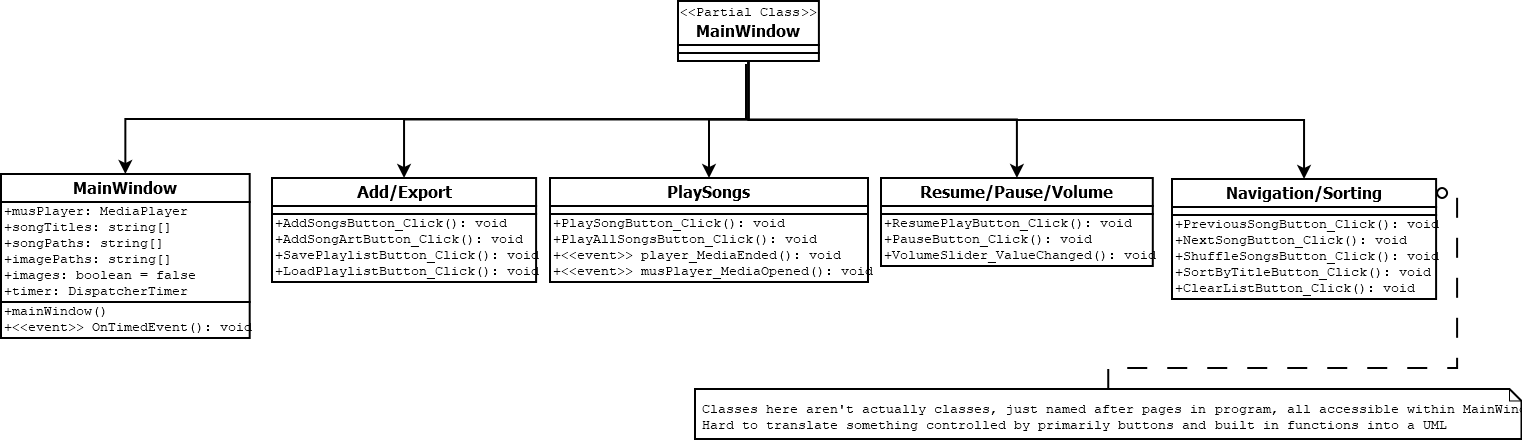
\includegraphics[height=250px, width=450px]{Manager_UML.png}
\caption UML outline of project, based off of implementation of functions and pages that are included in the program
\label{UMLOutline}
\end{figure}


\subsection{Design Patterns Used}
We decided to utilize two simple design patterns: and abstract factory pattern, and a decorator pattern (See Figure \ref{UMLOutline}). It would have been nice to try and use some more specific patterns, or ones that we had not practiced much, but it was difficult to work them into our project in a way that was useful, and couldn't just be implemented in a different, easier way. Even then, there were definitely other ways we could have gone about achieving the results of the patterns we used.
The abstract factory pattern provides basic light and dark themes, creating the grid background, toolbar, and song label items in the respective theme forms. We chose to use this pattern to make themes because it makes sense to have some theme options with an application like this. There are many more theme options that we could have made, or can still add later, but we settled on light and dark themes for the time being to prevent the GUI from getting too crowded.
The second pattern we used was a decorator pattern, which adds some more capability to the label that displays the name of the currently playing song. Normally the label would just show the user the name of the song, and updates as songs are changed. Using the decorator pattern, we added the ability to click the song label, which would change it from displaying the current song name, to displaying the song name, song path, and corresponding image path on the user's device. 
We thought this would be a useful way to implement the pattern, and it took the place of our original idea of playing a section of the song when the user selected it in the list. When trying to implement this first idea, we could not get the song to play for a set amount of time without having to use more libraries, which would have slowed the work down to the point where it would be too close for comfort on due dates, so we had to switch gears to this idea instead.


\section{Results}
Looking back on our ideas for the project when we were first brainstorming, we made some pretty lofty goals, and some of them were out of the scope of the time that we had, and the capabilities of Visual Studio. For example, we wanted to be able to save the last song listened to, and the time that was left in the song, so that the user could pick back up at the same place after closing the application, but this didn't seem easily accomplished within our work space, so we had to give up on the idea. Similarly, exporting music to a CD would require burning the CD, which ends up being a large stretch for the bounds of this project. All things considered, however, we did manage to get a lot of our use cases functioning, and meet most of our goals. If we had some more time to research, then I think we could definitely make some more progress towards our original vision.

\subsection{Future Work}
Unfortunately, the project will most likely not be making it's way out into the world, at least not anymore than it already is. It was a great way to practice what we've learned this semester, and to learn more about the capabilities of Visual Studio and WPF, but the project really doesn't put our best foot forward at this point, and doesn't have enough functionality that sets it apart from anything else that is already available. The manager may look good on a resume if either of us takes it further, and continues to work on it, but with the problems that we had finding time to work on it within the scope of this class, which gave us ample opportunity, it's unlikely that we'll have the free time to see it through to what we originally had hoped.

% that's all folks
\end{document}


